\chapter{Crypto.Symmetric.Tweakable\_Blockcipher}
Supposed that $M=m_1m_2m_3$, after encryption of normal block cipher (Chpater \ref{Blockcipher}) we get $C=c_1c_2c_3$, and if $m_1=m_3$, it is obvious that $c_1=c_3$, where $c=E(K,m)$. Thus the ciphertext may provide information about the plaintext.\\
For this reason a new block cipher type is considered by using a tweak value in key preparation, encryption or decryption, briefly $c=E(K,T,M)$. The tweak serves for much the same purpose that an initial vector for the CBC mode. Then if we encrypt the same plaintext block $m_1=m_3$ with the same key but distinct tweak values, we'll get two ciphertexts $c_1\neq c_3$ with a probability:
\begin{itemize}
\item $Pr[E(K,T,M)=E(K,T',M')]\approx \frac{1}{2^n}$
\end{itemize}
with $T\neq T', M=M'$, and $n$ is the size of the block. \\
This package is specified in \texttt{Crypto.Symmetric.Tweakable\_Blockcipher}.
\section{API}
\subsubsection*{Generic Part}
\begin{lstlisting}{}
  generic
    type Block is private;
    type Key_Type is private;
    type Tweak_Type is private;
\end{lstlisting}
\subsubsection*{Type}
\begin{lstlisting}{}
  type TB_Interface is limited interface;
\end{lstlisting}
If an interface is limited then it must be stated explicitly. This package provides a set of abstract operations with the interface \texttt{TB\_Interface}.\\
The API is made of the following operations:
\begin{itemize}
\item One procedure \texttt{Key\_Setup()} prepares a key.
\begin{lstlisting}{}
  procedure Key_Setup(This : in out TB_Interface;
                      Key  : in     Key_Type) is abstract;
\end{lstlisting}
\item One function \texttt{Encrypt()} encrypts a plaintext with a tweak value.
\begin{lstlisting}{}
  function Encrypt(This       : in out TB_Interface;
                   Tweak      : in     Tweak_Type;
                   Plaintext  : in     Block) 
                   return Block is abstract;
\end{lstlisting}
\item One function \texttt{Decrypt()} decrypts a ciphertext with the tweak value.
\begin{lstlisting}{}
  function Decrypt(This       : in out TB_Interface;
                   Tweak      : in     Tweak_Type;
                   Ciphertext : in     Block) 
                   return Block is abstract;
\end{lstlisting}
\end{itemize}
\textbf{Notice that these operations are all abstract, they have no body and can never be called.} An implementation of the abstraction can be created by deriving a concrete type from the interface \texttt{TB\_Interface} and providing concrete operations for that implementation. Figure \ref{TweakBlock} shows the general structure of a tweakable blockcipher.
\begin{figure}[htp]
\centering
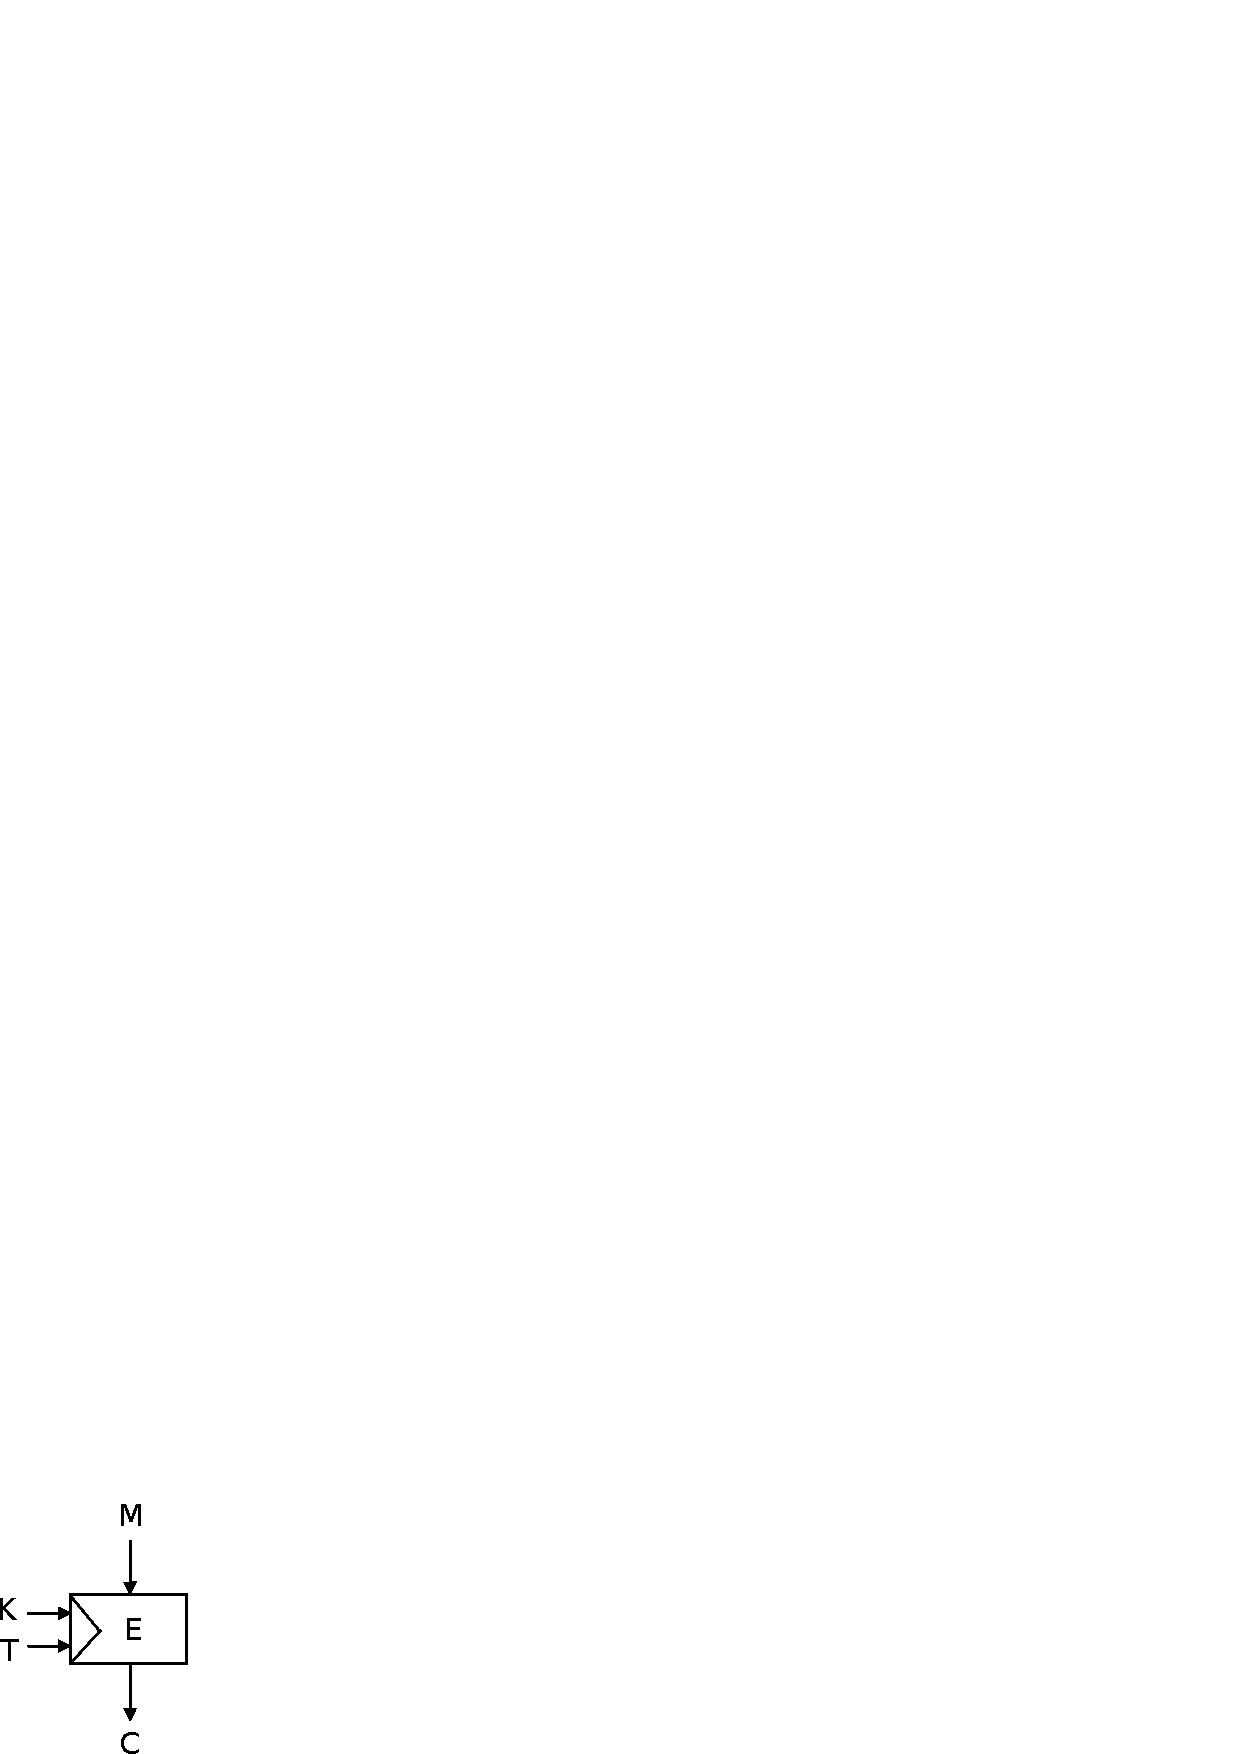
\includegraphics[scale=1]{Pictures/Tweak_BC.pdf} 
\caption{Structure of the tweakable blockcipher.}\label{TweakBlock}
\end{figure}
%%%%%%%%%%%%%%%%%%%%%%%%%%%%%%%%%%%%%%%%%%%%%%%%%%%%%%%%%%%%%%%%
%%%%%%%%%%%%%%%%%%%%%%%%%%%%%%%%%%%%%%%%%%%%%%%%%%%%%%%%%%%%%%%%
\section{Child Packages}
The ACL provides two instantiations of the tweakable block cipher. The two tweakable block cipher based implementations can be distinguished by the usage of the tweak value. The package \texttt{Tweakable\_Blockcipher\_TX} uses the tweak value in key preparation, while in the package \texttt{Tweakable\_Blockcipher\_CMT} the tweak value is used in encryption. Other instantiations of the tweakable block cipher will be provided in the future.
\subsection*{Tweakable\_Blockcipher\_TX}
\subsubsection*{Generic Part}
\begin{lstlisting}{}
  generic
    with package BC is new Crypto.Symmetric.Blockcipher(<>);
    with function To_Bytes(K : in BC.Key_Type) 
    								return Crypto.Types.Bytes;
\end{lstlisting}
\subsubsection*{Types}
\begin{lstlisting}{}
  package Tweakable_Blockciphers is new
   Crypto.Symmetric.Tweakable_Blockcipher(Block   	  => BC.Block,
														Key_Type   => BC.Key_Type,
														Tweak_Type => BC.Block);
   type TX is new Tweakable_Blockciphers.TB_Interface with private;
\end{lstlisting}
\subsubsection*{Procedures}
Concrete operations are provided here for the concrete type TX to implement the interface \texttt{TB\_Interface}.
We have to include the \texttt{overriding} indicator whenever we declare a further \texttt{Key\_Setup()}, \texttt{Encrypt()} or \texttt{Decrypt()}. This ensures that if we make a simple typographical error such as misspelling or getting the parameters wrong then the compiler will detect the error and not just add a bogus operation.
\begin{lstlisting}{}
  overriding
  procedure Key_Setup(This : in out TX; Key : in BC.Key_Type);
  overriding
  function Encrypt(This       : in out TX;
                   Tweak      : in     BC.Block;
                   Plaintext  : in     BC.Block) return BC.Block;
\end{lstlisting}
Function \texttt{Encrypt()} calls the procedure \texttt{Key\_Setup()} to combine the value \texttt{Tweak} and a user-defined key in order to generate a cipher key, and then encrypts the plaintext under the cipher key. By decryption it makes from the value \texttt{Tweak} a cipher key and then use this key to recover the ciphertext.
%%%%%%%%%%%%%%%%%%%%%%%%%%%%%%%%%%%%%%%%%%%%%%%%%%%%%%%%%%%%%%%%%%%%%%%%
%%%%%%%%%%%%%%%%%%%%%%%%%%%%%%%%%%%%%%%%%%%%%%%%%%%%%%%%%%%%%%%%%%%%%%%%
\subsection*{Tweakable\_Blockcipher\_CMT}
\subsubsection*{Generic Part}
\begin{lstlisting}{}
  generic
    with package BC is new Crypto.Symmetric.Blockcipher(<>);
    with function "xor"(Left, Right: BC.Block) return BC.Block is <>;
\end{lstlisting}
\subsubsection*{Types}
\begin{lstlisting}{}
  package Tweakable_Blockciphers is new
   Crypto.Symmetric.Tweakable_Blockcipher(Block      => BC.Block,
														Key_Type   => BC.Key_Type,
														Tweak_Type => BC.Block);
   type CMT is new Tweakable_Blockciphers.TB_Interface 
   											with null record;
\end{lstlisting}
Concrete operations should be provided for the new interface \texttt{CMT}.
\subsubsection*{Procedures}
\begin{lstlisting}{}
  overriding
  function Encrypt(This       : in out CMT;
                   Tweak      : in     BC.Block;
                   Plaintext  : in     BC.Block) return BC.Block;
\end{lstlisting}
In the procedure \texttt{Encrypt()} the encryption process will be made twice. After the first encryption the ciphertext is XORed with the value \texttt{Tweak} and then delivered as plaintext for the second time. In the procedure \texttt{Decrypt()} vice versa.\\
%%%%%%%%%%%%%%%%%%%%%%%%%%%%%%%%%%%%%%%%%%%%%%%%%%%%%%%%%%%%%%%%%%%%%%
%%%%%%%%%%%%%%%%%%%%%%%%%%%%%%%%%%%%%%%%%%%%%%%%%%%%%%%%%%%%%%%%%%%%%%
\section{Example}
\begin{lstlisting}{}
  with Crypto.Symmetric.Tweakable_Blockcipher_CMT;
  with Crypto.Symmetric.Blockcipher_AES128;
  with Crypto.Types;
  with Crypto.Types.Random;
  with Ada.Text_IO;
  procedure Example_TBC is
    package AES128 renames Crypto.Symmetric.Blockcipher_AES128;
    package CMT128 is new Crypto.Symmetric.Tweakable_Blockcipher_CMT
   					 (BC => AES128, "xor" => Crypto.Types."xor");
    use CMT128;
    use Crypto.Types;
    TB_CMT : CMT128.CMT;
    Key, P_1, P_2 : B_Block128;
    Ciphertext : B_Block128;
    Tweak_Value : B_Block128;
  begin
    Crypto.Types.Random.Read(P_1);
    Crypto.Types.Random.Read(Tweak_Value);
    Key_Setup(TB_CMT, Key);
    Ciphertext := Encrypt(TB_CMT, Tweak_Value, P_1);
    P_2 := Decrypt(TB_CMT, Tweak_Value, Ciphertext);
    if P_1 = P_2 then
       Ada.Text_IO.Put_Line("Same");
    end if;
  end Example_TBC;
\end{lstlisting}